\externaldocument{1-introduction}

\chapter{Generic Offline Design}\label{chap:offline}
The implementation of distributed assertion checking on any blockchain requires some off-chain considerations and infrastructure. The previous chapter defined a formal set of logical formulae amenable for this approach and gave some in-depth examples. As stated before, the proposed implementation in the following chapters is, for the most part, restricted to formulas of predicate logic using universal quantification.\\
The purpose of the offline infrastructure is to provide a syntax for stating assertions that check logical formulas, as well as a toolchain to compile these assertions into code that can be originated on the target blockchain. Depending on the individual solution for the respective blockchain protocol, this can either be the original contract extended directly with the assertion code, or as a separate contract that extends the original contract in some other way. This chapter describes the generic part of the offline design, which corresponds to the frontend of the compilation pipeline shown in \figref{fig:pipeline_frontend}. As a start, \secref{sec:syntax} describes the concrete syntax for writing assertions and shows how it expresses some of the previously given examples. The stages of the pipeline frontend, including parsing and transforming the original assertions to assertions that check for counterexamples, are described in \secref{sec:pipeline_front}. Lastly, \secref{sec:accuracy} analyses the reliability of distributed assertion checking as proposed and the cost incurred by increasing it.

\section{Assertion syntax}\label{sec:syntax}
The assertion syntax is described in two versions by the EBNF grammars shown in appendix \ref{apx:grammar}. One version implements a prefix and the other one an infix notation. The pipeline currently supports the prefix notation with mandatory parentheses to avoid the need of handling operator precedences. To avoid context switches (at least for developers on Tezos), the assertion syntax references those of OCaml and thereby also Michelson.\\
A file containing assertions (henceforth referred to as ``assertion contract'') contains at least one assertion for some function or entrypoint of the original contract (henceforth referred to as ``parent contract''). An assertion begins with a signature consisting of an optional tag followed by a parameter type declaration. The tag can be used for documentation, but may sometimes be needed to indicate to which function of the parent contract the assertion should be assigned. The body is an (optional) nesting of quantifiers and conditions around exactly one assertion. Conditionals can be used to restrict the quantification domains or for some other constraints. For completeness, the existential quantifier is already included in the grammar, however the current version of the pipeline will reject any assertions containing it. \\
In order to make the frontend generic, the assertion grammar constitutes a union of operations and types for the target languages. This also allows the transformation to be oblivious of the target platform and be identical for all backends. The current version of the grammar recognizes all types present in the Tezos VM and a subset of operations that Michelson provides ( \secref{sec:tezos} contains an introduction to Tezos and Michelson and goes more into detail about this). Responsible for rejecting any assertions containing unsupported types or operations are the respective backends.\\

As an example, consider a variation of the formula given in \eqref{eq:sorted} that checks whether a given list is sorted in ascending order:
\begin{equation}\label{eq:sorted_v2}
	(\forall n : int)(\forall m : int) (0 \leq n < m < |a|) \Rightarrow a[n] \leq a[m]
\end{equation}
The respective assertion that checks this property for the parent contract from \lstref{lst:sorted} could be expressed as follows:
\lstinputlisting[caption=Assertion contract for checking if a list is sorted, language=Assertion, label={lst:sorted_assertion}]{listings/sorted.tza}

\subsection{Extensions}
In future iterations, the assertion syntax could be extended with some more features to improve usability and readability:
\begin{itemize}
\item \textbf{Local variables} to store, reuse and denominate computed values
\item \textbf{User-defined functions} to extract whole routines that can be reused in a single or even many assertion contracts, if defined as a module.
\item \textbf{if-else conditions} to adapt the domains of quantifications if certain conditions hold. The assertion that checks whether two numbers are relatively prime (discussed in \secref{sec:coprime}) is a good use-case for this feature: Firstly, the minimum of the given number has to be determined, however the \texttt{min}-function might not be supported as a built-in function by the target language (Tezos, for instance, does not support it). A solution for that could be to implement two branches in the program to handle each case. Secondly, if the greater of the two numbers is not evenly divided by the smaller one, the formula can be optimized by reducing the quantification domain by half to $(2 \le n \le \lfloor \frac{min(a,b)}{2} \rfloor)$, as a number cannot be evenly divided by any number between itself and its half \cite{bernhardt_veigel_2020}. With a syntax supporting an \texttt{if-else} control structure, the optimized assertion could look as follows:
\lstinputlisting[caption=Assertion syntax with if-else structures \cite{bernhardt_veigel_2020}, language=Assertion, label={lst:coprime}]{listings/coprime_ifelse.tza}
This feature is not included in the current version, because conditional domain restrictions make the translation from quantifiers to random generators or loops more complex. Aside from that, without the feature of variables and user-defined functions, the code is inflated significantly, thus causing increased origination cost.
\end{itemize}

\section{Frontend of the pipeline}\label{sec:pipeline_front}
The frontend of the compilation pipeline comprises of a command-line interface (CLI), a parser and the transformation. These stages are generic and independent of the target platform and produce an abstract syntax tree (AST) of the assertion that is passed to the respective back-end through a public interface.
\begin{figure}[h]
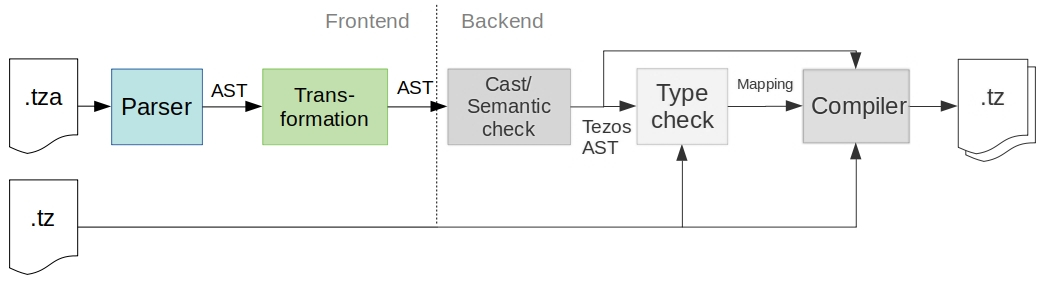
\includegraphics[width=\linewidth]{figures/3-offline/pipeline_frontend}
\caption{The stages of the generic frontend of the compilation pipeline}
\label{fig:pipeline_frontend}
\end{figure}
OCaml was chosen as a programming language to implement the pipeline, given that it's also used to develop the Tezos blockchain refer to \secref{sec:tezos}). This avoids context switches within the Tezos eco-system and allows to build on top of the Tezos libraries. \chapref{chap:offline_tezos} goes into more details about this.

\subsection{Parser}
Assertions expressed in the syntax described above are passed as a simple text file to the pipeline. The file extension is irrelevant, but this thesis follows the convention of using the file extension \texttt{.tza} for assertion contracts (referring to the extension \texttt{.tz} for Michelson contracts). The file must contain at least one assertion, hence it is not admissible to create empty assertions for all functions (or entrypoints) of the parent contract. Furthermore, every syntax error will cause the pipeline to abort execution in order to ensure that no assertion is missing in the target code. Each of the contained assertions is, after parsing, represented as a separate abstract syntax tree (AST). The AST represents, like the syntax itself, a union of all target specific ASTs that contain the supported subsets of operations and types. \\
Both lexer and parser have been generated using the OCaml tools \texttt{ocamllex} \cite{ocaml_docs} and \texttt{menhir} \cite{menhir_doc}.

\subsection{Transformation}\label{sec:transformation}
Since the validators will check the input parameter for the negation of the formula, it has to be transformed before compilation. Furthermore, the formula should explicitly state the domain for each quantifier, which will have to be translated into a set of bounds that refer to the respective random generator. Restricting the ranges of the random generators is important in order to avoid wasting resources through testing values out of the relevant (or legal) scope.

\subsubsection{Negation}
The formula is negated using the negation rules of second-order logic and applying De Morgan's laws \cite{de_morgan} until the negation is applied to the literals. Negating universal quantification is equivalent to an existential quantification of its negated body (and vice versa): $\neg \forall x P(x) \equiv \exists x \neg P(x)$ \cite{Sundstrom2020Quantifiers}. The domain restrictions are not affected by the negation, which is also reflected in the rules of predicate logic if the domain is given as a premise in the logical formula: $\neg (p \Rightarrow q) \equiv p \Rightarrow \neg q $.

\subsubsection{Building smart random generators}
In order to assign each explicit bound to its appropriate quantifier, the formula has be skimmed for atomic constraints that contain predicate (bound) variables. They're then moved and assigned to the quantifier that bounds the variable. If the constraint contains more than one bound variable, it is assigned to the quantifier with the highest depth in the order of quantifiers, as they depend on the generated value(s) of the other variable(s). \\
Revisiting the formula from \eqref{eq:sorted_v2}, its premise can be considered as a conjunction of the four constraints
\begin{itemize}
\itemsep-1em
\item $0 \leq n$
\item $n < |a| $
\item $n \le m$ and
\item $m < |a|$.
\end{itemize}
Applying the rules given above after negating the formula, the constraints are assigned to the quantifiers as follows:
\begin{equation}\label{eq:sorted_v2_bounds}
	(\exists n : int, 0 \leq n \wedge n < |a|])(\exists m : int, m > n \wedge m < |a|) \text{ } a[n] > a[m]
\end{equation}
Ultimately, the quantifiers are then translated to the corresponding random generators, drafted in pseudocode:
\begin{lstlisting}[label=lst:rand, numbers=none]
n = random(0, size(list))
m = random(n, size(list))
\end{lstlisting}
While conjunctions can be handled easily, other operators make it more difficult to derive efficient random generators. Consider the following constraints:
\begin{itemize}
\itemsep-0.7em
\item[1)] $(\forall n : int) (n < 10 \lor n > 20) ...$
\item[2)] $(\forall n : int) (n \ne 10) ...$
\item[3)] $(\forall n : int) (n = 10) ...$
\end{itemize}
Constraint 1) complicates restricting the random generator in several ways. Firstly, it separates the domain into two disjoint sub-domains, which requires defining a random generator for each range and another one to decide which one is called. Secondly, the operands of a disjunction cannot be considered separately when more than one bound variable is involved. For the predicate variable whose random generator is executed first, the domain restriction is optional, while the generation of the following random values depend on the previous result. Similarly to 1), constraint 2) splits the domain into sub-domains. To keep it simple for the time being, restrictions formulated with these operators are kept as part of the assertion code rather than used as constraints for the generators. Consequently, some validators may generate irrelevant values when checking the assertion and, depending on the size of the gap between the sub-domains, this can significantly decrease the reliability of this kind of assertion checking. Thus, further developed iterations should handle and translate them accordingly.\\
Constraint 3) effectively makes the quantifier, which binds $n$, obsolete. Adding this constraint to the respective generator will at least not affect the reliability, but a future improvement could be to optimize the assertion by replacing all occurrences of the bound variable with the assigned value and removing the quantification.

\subsubsection{Implicit constraints}
In some cases, boundaries are imposed implicitly by data types. List indices, for instance, are always bound to the range $0.. size(list) - 1$ and could thus be derived from the formula without an explicit specification. As this deduction makes the transformation more complex, requiring a semantic analysis of the formula, a completely explicit formula in terms of the domain is required for now. Depending on the VM, the lower bound for indexing operations can be implicitly handled by the random generator of an appropriate predicate type. As an example, Michelson supports the data type \texttt{nat} representing the natural numbers, which categorically excludes all values below zero. Developers aware of this can exploit this and, for instance, abbreviate \eqref{eq:sorted_v2} with the following formula:
\begin{equation}\label{eq:sorted_v2_abbr}
	(\forall n : nat)(\forall m : nat) (n \le m < |a|) \Rightarrow a[n] \leq a[m]
\end{equation}

\section{Accuracy of the approach}\label{sec:accuracy}
Since the proposed approach implements a probabilistic test, the accuracy as well as the costs incurred by guaranteeing a specified certainty threshold, need to be examined closely. The goal is to identify a formula that, given the domain of a formula in predicate logic, returns an estimate of a lower bound of samples necessary to find an existing counterexample with a probability $p$. From this analysis, it can be derived how effective a formula can be checked on a blockchain with $m$ validators. Sections \ref{sec:coupon} and \ref{sec:prob_threshold} depict the findings from \cite{bernhardt_veigel_2020} and are based on the assumptions that the random generator picks elements independently from a uniform distribution and that there exists exactly one counterexample for the passed parameter.

\subsection{Coupon Collector's Problem Analysis}\label{sec:coupon}
When checking properties with probabilistic testing, the result is either definitely not satisfied, or probably satisfied. Thus, errors only occur as false positives. In order to find an existing counterexample with probability $p = 1$, every element in the given domain $\mathcal{D}$ has to be checked by at least one validator. Deterministically, this is reachable with exactly $|\mathcal{D}|$ test runs. This is, however, invalid for the probabilistic approach, as some validators may generate duplicate random values and leave some elements of $\mathcal{D}$ unchecked. \\
In probability theory, this is known as the Coupon Collector's Problem \cite{croucher_collecting_2006}. Given $n = |\mathcal{D}|$, the probability that no duplicate elements are generated with $n$ picks is given by
\begin{equation*}
    p = \prod_{i=1}^{n} \frac{i}{n}
\end{equation*}
As an example, the probability that all validators generate a unique random value already drops to $0.036\%$ for $n = 10$. Let the random variable $T$ be the number of test runs executed until every element in the domain has been generated. In order to obtain an estimation of how many test runs are needed to find the counterexample for certain, the goal is to identify its expectation $E(T)$. To this end, the geometric probability distribution is applied \cite{croucher_collecting_2006}:\\
Each element is generated with a probability of $1/n$. Thus, the probability to generate the $i$th unique element is given by 
\begin{equation}
    p_i = \frac{n-i+1}{n}
\end{equation}
\cite{croucher_collecting_2006}. The expected value of a random variable $X$ is given by $E(X) = \frac{1}{p}$\cite{croucher_collecting_2006}, thus the expected number of test runs for $n$ is 
\begin{equation}
E(T) = n \sum_{i=1}^{n} \frac{1}{i}
\end{equation}
\tabref{tab:prob_outcomes} shows the expected number of test runs $E(T)$ and its standard deviation $\sigma$ for different $n$. Furthermore, $E(T)$ and $\sigma$ are used to calculate a 95\% confidence interval for $T$ by applying the central limit theorem, which provides an upper and lower bound on the number of test runs \cite{croucher_collecting_2006}. Rounded values for both bounds are also shown in \tabref{tab:prob_outcomes}.
\begin{table}[h]
    \centering
    \begin{tabular}{lllll}
        \thead{$n$} & \thead{$E(T)$} & \thead{$\sigma$} & \thead{lower bound} & \thead{upper bound}\\ \hline
        5 & 11.4 & 2.53 & 6 & 16\\
        10 & 29.3 & 4.32 & 21 & 38\\
        20 & 72.0 & 7.21 & 58 & 86\\
        30 & 119.8 & 9.48 & 101 & 138 \\
        50 & 225.0 & 13.23 & 199 & 251 
    \end{tabular}
    \caption{Expectation, standard deviation and upper and lower bound of needed test runs for some $n$ \cite{croucher_collecting_2006}}
    \label{tab:prob_outcomes}
\end{table}

The results show that checking random values is a very inefficient approach if false positives are not admissible. Even if the lower bound of $T$ is chosen as the number of test runs, it exceeds the size of the domain by far and increases the time complexity to $\mathcal{O}(n*log(n))$ for large $n$ \cite{xu_tang_2011}. For instances where false positives are tolerable, the following section introduces a formula to calculate the number of test runs that detect counterexamples with a given probability threshold $p \leq 1$.

\subsection{Setting probability thresholds}\label{sec:prob_threshold}
The goal is to find a number $t$ of test runs, s.t. the probability $P_{c,t}$ of not finding the counterexample drops below a certain threshold $c$. A validator finds the counterexample in one test run with probability $\frac{1}{n}$, and misses it with probability $(1-\frac{1}{n})$. After $t$ tests runs, the probability that the counterexample has not been found is thus $(1-\frac{1}{n})^t$. Following the same approach as in \cite{mahl_schindel_2007} to retrieve an upper bound for $P_{c,t}$, we use the following inequality
\begin{equation}
(1-\frac{1}{m})^m \leq \frac{1}{e}
\end{equation}
which holds for all $m > 0$. From this inequality, it follows that
\begin{equation}
(1-\frac{1}{n})^t = ((1-\frac{1}{n})^n)^{\frac{t}{n}} \le e^{-\frac{t}{n}}
\end{equation}
With this, the probability $P_{c,t}$ of not finding the counterexample with $t$ test runs can be defined as
\begin{equation}
P_{c,t} \le e^{-\frac{t}{n}}
\end{equation}
In order to retrieve the number of test runs $t$ necessary for $P_{c,t}$ to drop below a specified threshold $c$, the inequality is solved for $t$, which is then dependent of the known parameter $n$ and an arbitrary value for $c$:
\begin{align}
    e^{-\frac{t}{n}} &\leq c && \text{with } 0 \leq c\le 1 \nonumber\\
    t &\geq -n\:\ln(c)
\end{align}
For $c = \frac{1}{e}$ ($\approx 36.79\:\%$) the lower bound of $t$ is exactly $n$, which means that for higher reliabilities the number of test runs needs to be greater than $n$. \figref{fig:graph_t_c} shows the lower bounds of $t$ as a function of the probability threshold and domain size. One can see that the increase in accuracy is approximately linear to the number of test runs below a threshold of $c=0.5$, but requires an exponential testing effort to reach higher thresholds.
\begin{figure}[h]
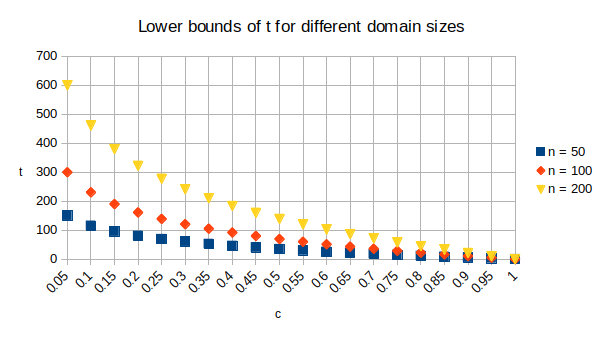
\includegraphics[width=0.95\linewidth]{figures/3-offline/graph_t_c}
\caption{The number of required test runs as a function of the probability of false positives $c$ and size of the domain $n$}
\label{fig:graph_t_c}
\end{figure}
For assertions with several quantifiers, which are translated to random generators, all domains have to be considered in the calculation. Revisiting the intersection of sets from \secref{sec:existential}, every element in set $U$ has to be compared to every element in set $V$. Thus, the lower bound of test runs needed to check whether they intersect with a certainty of 63.21\% is given by $t \leq t_1 * t_2$ with $t_1 \geq |U|$ and $t_2 \geq |V|$.

\subsection{Validators vs. test runs}
The last section derived a formula to calculate a lower bound for a number of test runs $t$ in order to reach a certain level of confidence. However, $t$ is not a parameter that can be adjusted to an arbitrary value on the blockchain, as the assertion is checked by the validators. Assuming a blockchain has $m$ validators, the actual lower bound of test runs is $m$. For cases where there are not enough validators to reach a threshold $c$, a mechanism is required to have each validator check the property for multiple random values. Hence, the actual executed number of checks is always a multiple of $m$. \secref{} goes into a bit more detail about this based on the Tezos blockchain. \todo{Refer to section}

\subsection{Alternatives to random testing}\label{sec:alt_random}
For applications where higher reliability is crucial, an alternative to checking elements randomly could be to coordinate a systematic iteration of the domain. The implementation of such a coordination is not trivial though; validators can't simply be passed an individual value as input. Instead, possible approaches could be to implement a central instance that allocates an element in the search space to each validator, or use some unique and intrinsic attribute, like an identification number, as input for a mapping. The discussion if this approach would provide any advantages over a local validation of the property is left open \todo{Depends on cost analysis?}.

\subsubsection{Central instance assigning values}
For this approach, the tool-chain would need to generate a separate contract that is called by the miners and validators as a proxy. This contract would then, for instance, generate a number using a modulo-n counter and pass this number as an additional parameter to the assertion code. The random generators would be omitted accordingly. However, this works only as expected if there are no simultaneous transactions calling the contract, otherwise it cannot be guaranteed that all elements have been checked for each of the transactions. If and how this issue can be solved will not be discussed further in this thesis.
\todo{Serializes tests -> see expose rejected ideas}

\subsubsection{Using unique attributes of a validator}\label{sec:alt_attributes}
This approach strongly depends on whether the validators have a unique id or other attribute that can be accessed from within a contract.  If there is (or the language can be extended with such a feature), there needs to exist a non-injective surjective function that maps the respective attributes represented by type A to an element of the domain represented by type B, i.e. $f: X \rightarrow Y$. Furthermore, for cases where $t > m$, an offset needs to be added, s.t. a validator checks distinct elements for each test run. \\
Implementing such an approach on Tezos becomes even more challenging due the way endorsing (i.e. validation) rights are distributed in its proof-of-stake mechanism: for each block level, endorsing rights are assigned to the owner of a randomly selected roll, i.e., a set of tokens \cite{tezos_docs}. This means that the same validator can be picked multiple times for endorsing one block and thus some elements in the domain may remain unchecked. \secref{} goes into more detail about this issue. \todo{Ref section}